\section{Energy Efficiency of High Order Finite Element Kernels}
\label{sec:section2}

This section describes ongoing work in task WP3.4 on energy and performance profiling.
The object of study is the matrix-free evaluation of high-order finite element operators, i.e.\ the kernels that dominate the run time of implicit and explicit high-order solvers.
These kernels are characterised by a small arithmetic footprint per degree of freedom at low polynomial degree and a rapidly growing one at high degree, so that the same operator traverses the memory-bound and the compute-bound regime as the degree is varied.
The degree is not merely a runtime parameter, however: efficient implementations specialise for it, through C++ templates or through just-in-time compilation, so that each degree is in effect its own generated code.
This makes the family a convenient probe of the energy behaviour of a node, and it also places the code-generation strategy and the compiler among the parameters under study rather than outside them.

The motivation is one of scale.
A single NVIDIA H100 held at 61\,\% of its 700\,W thermal design power over a full year consumes
%
\[
  0.700\,\mathrm{kW} \times 0.61 \times 8760\,\mathrm{h} \approx 3740\,\mathrm{kWh},
\]
%
which is more than the 3500\,kWh of the reference household commonly used in German electricity statistics, and this is the bare accelerator, before cooling, the host and the rest of the node are accounted for.
A production system aggregates tens of thousands of such devices: JUPITER drew close to 16\,MW during its exascale TOP500 run, with an average operational demand estimated at some 11\,MW, which over a year is of the order of the household electricity consumption of a small town.
At this scale the Joules spent by a kernel are a first-order concern, and energy-conscious HPC --- treating energy-to-solution as a figure of merit on the same footing as time-to-solution --- becomes a design constraint on codes and not only on machines.
This is the perspective from which the present task approaches EuroHPC systems.
% Sources: BDEW reference household 3500 kWh, cf. https://www.cleanenergywire.org/factsheets/what-german-households-pay-electricity
% JUPITER 15.87 MW (TOP500 Nov 2025); 11 MW average estimate, FZJ press release
% https://www.fz-juelich.de/en/news/archive/press-release/2024/european-exascale-supercomputer-jupiter-sets-new-energy-efficiency-standards-with-1-ranking-on-green500

The massive parallelism and comparatively low clock frequency of GPUs can offer significant advantages for scientific codes in comparison to CPUs.
Power, however, grows super-linearly with frequency, so the operating point that minimises time-to-solution is in general \emph{not} the one that minimises energy-to-solution.
Quantifying the gap between the two, for a kernel class of practical relevance, is the purpose of this task.

\subsection{Metrics}

Energy-to-solution is, by definition, the integral of the instantaneous power dissipation over the measured interval,
%
\begin{equation}
  E = \int_{0}^{T} P(t)\,\mathrm{d}t .
\end{equation}
%
The power dissipation $P$ can in principle be modelled as a function of clock frequency and of the achieved performance, and there is a substantial literature doing so.
This is deliberately not the route taken here.
Within WP3.4 we measure $E$ directly and proceed empirically, with the aim of establishing where our kernels currently stand and what can be gained by tuning them, rather than of producing a predictive power model.

Performance is reported as the number of degree-of-freedom updates per second (GDoF/s), the customary throughput metric for matrix-free operator evaluation.
Energy efficiency is reported as the number of \emph{DoF updates per Joule}, which is simply the throughput normalised by the average power drawn during the measured region,
%
\begin{equation}
  \eta = \frac{\text{DoF updates}}{E} = \frac{\text{DoF updates}/t}{\bar{P}} .
\end{equation}
%
Reporting $\eta$ alongside GDoF/s makes the trade-off explicit: a configuration that is faster but disproportionately more power-hungry shows up immediately as a loss in $\eta$.

Where a single figure of merit is needed, the energy--delay product $\mathrm{EDP} = E\,t$ is used as a secondary metric.
It exists because energy on its own is a manipulable objective: on most devices energy-to-solution can be reduced simply by clocking down and running longer, up to the point at which static power begins to dominate, so a criterion counting only Joules would endorse operating points that nobody would choose to run in production.
Multiplying by the delay penalises exactly that.
Normalised per DoF update, and with $N$ the number of DoF updates, the product reads
%
\begin{equation}
  \frac{E\,t}{N^{2}} = \frac{1}{\eta\,R} ,
\end{equation}
%
so minimising it is the same as maximising the product of energy efficiency $\eta$ and throughput $R$.
It is therefore not an independent measurement but the single number that follows from the two curves we already report.
Weighting energy and delay equally is a convention, and the variant $\mathrm{ED^{2}P} = E\,t^{2}$, which weights time-to-solution more heavily, is also in common use.
The exponent that is appropriate for a given site follows from the ratio of its energy cost to its machine-time cost, and we therefore report $\eta$ and $R$ separately throughout and use the energy--delay product only as a summary.

\subsection{Measurement methodology}

Measurements are driven by \texttt{p3em}, our in-house approach to power, performance and energy measurement.
Rather than wrapping the benchmark binary as a whole, it instruments a local scope of the program: a background thread queries a power meter running as a separate process, over a rudimentary client--server interface, and integrates the returned power readings over the lifetime of the scope.
Two properties of this design matter for the study.
First, it is selective: the measured region can be restricted to the parts of the program that are of interest, such as the operator evaluation, the preconditioner or the solve, while excluding I/O and set-up phases that would otherwise dilute the result.
Second, it is portable, since support for a new machine requires only a different meter script, the rest of the instrumentation being unchanged; in the common case the whole chain runs in user space, without privileged access.

The approach is not specific to the kernels studied here.
It has been applied to a set of flagship science applications on SuperMUC-NG Phase~2, in a study presented at the IXPUG workshop of ISC~2026 which documents the methodology and its validation in more detail.\footnote{%
  \emph{Node-Level Performance and Energy Characterization of Flagship Science Applications on SuperMUC-NG Phase~2}, IXPUG workshop, ISC~2026, Hamburg, 26 June 2026.
  Preprint: \texttt{arXiv:2606.23265}.%
}
That work measures whole applications rather than isolated kernels, and is the natural counterpart to the kernel- and problem-level measurements reported below.

Around this instrumentation, the study of a given system consists of the following components.
%
\begin{itemize}
    \item Investigating the operating points exposed by the device and by the host: the clock frequencies the hardware supports and the range over which they may be set, together with any power-cap and memory clock settings that are available.
    \item Setting an operating point and running the kernel sweep (polynomial degree, number of elements, precision) with the instrumented region active.
    \item Recording one entry per (kernel, degree, operating point) tuple, so that performance and energy come from the same run and are directly comparable.
\end{itemize}
%
The meter scripts build on NVML on NVIDIA devices, the AMD SMI library on AMD devices, and the Level~Zero sysman interface on Intel devices.
Three methodological points require care and are documented together with the results: the sampling rate of the meter and its latency relative to short measured regions, the treatment of idle power, and the attribution of energy on tightly coupled packages such as the GH200 superchip, where the CPU, the GPU and the memory share a configurable power budget.

Systematically analysing power limits and frequency settings in this way allows the project to make informed decisions about optimising energy efficiency while maintaining a satisfactory level of performance, and to state the cost of that trade-off in concrete terms, e.g.\ the energy saved at a prescribed loss in time-to-solution.

Tables~\ref{tab:nvidia} and~\ref{tab:amd} collect the devices of interest.
The quoted thermal design power should be read with caution: vendors give a single number, obtained under an unspecified workload, and it is an indication of the class of the device rather than a bound that our measurements can be compared against.
The figures that are directly actionable for this study are instead the frequencies the device supports and the range over which they can be set, which is what the sweeps of Section~\ref{sec:wp34plan} vary.

% EuroHPC GPUs
%---------------------------
% JUPITER - GH200
% LUMI - AMD EPYC + AMD Instinct MI250X
% LEONARDO - Intel Xeon (ICX, SPR) + Nvidia Ampere "Da Vinci"
% MARENOSTRUM5 - Intel Xeon (SPR) + Nvidia Grace + Nvidia H100
% MELUXINA - AMD EPYC + Nvidia Ampere A100
% KAROLINA - AMD EPYC, Intel Xeon + Nvidia A100
% VEGA - AMD EPYC + Nvidia A100
% DISCOVERER - AMD EPYC + Nvidia DGX H200
% DEUCALION - Arm A64FX, AMD EPYC, Nvidia A100
% DAEDALUS - Nvidia GH200
% ARRHENIUS - AMD EPYC Turin, GH200
% ALICE RECOQUE - AMD EPYC Venice + AMD Instinct MI430X

\begin{center}
\begin{table}[h!]
\centering
\small
\caption{Characteristics of the Nvidia and Intel GPUs of interest}
\label{tab:nvidia}
\medskip
\begin{tabular}{l|cccc}
                      & A100  & H100 NVL & GH200           & Intel Data Center GPU Max 1550 \\ \hline
TDP [W]               & 440   & 350-400  & 680 (superchip) & 600    \\
FP32 [TFLOPS]         & 22.4  & 60       & 67              & 52.4   \\
Bandwidth [TB/s]      & 1.64  & 3.9      & 4               & 3.2    \\
Base Frequency [MHz]  & 1245  &          &                 & 900    \\
Boost Frequency [MHz] & 1395  &          &                 & 1600   \\
Memory Size [GB]      & 64    & 64       & 96              & 128    \\
Memory Type           & HBM2  & HBM2e    & HBM3            & HBM2e  \\
\end{tabular}
\end{table}
\end{center}
% TODO: check the memory sizes. The A100 ships as 40 GB or 80 GB and the
% H100 NVL as 94 GB HBM3 (NVIDIA product brief PB-11773-001); 64 GB does not
% correspond to a catalogue part for either.
% TODO: base/boost frequencies missing for H100 NVL and GH200 -- these are the
% quantities the frequency sweeps act on, so they are worth completing.

% A100 data is provided for the system in LEONARDO (CINECA)
% The values are taken from the work
%  https://jlsrf.org/index.php/lsf/article/view/186/345
% Frequencies for the A100 are taken from the work of Amati and Turisini,
%  https://arxiv.org/pdf/2406.11498

% H100 data is taken for Marenostrum5
%  https://arxiv.org/pdf/2503.09917v1

% GH200 data for JUPITER Booster
% https://www.fz-juelich.de/en/jsc/jupiter/tech
% https://apps.fz-juelich.de/jsc/hps/jupiter/configuration.html#jupiter-booster-design
%
% In general GH200 power is configurable from 450 to 1000 (Memory + CPU + GPU)
% https://nvdam.widen.net/s/rrgqqnpbz8/grace-datasheet-gh200-grace-hopper-superchip-3773000%20

\begin{center}
\begin{table}[h!]
\centering
\small
\caption{Characteristics of AMD GPUs of interest}
\label{tab:amd}
\medskip
\begin{tabular}{l|ccc}
                          & AMD MI250X & AMD MI300X & AMD MI430X  \\ \hline
TDP [W]                   & 500        & 750        & 2500 (est.) \\
Peak Performance [TFLOPS] & 47.9       & 81.72      & 288 (fp64)  \\
Peak Bandwidth [TB/s]     & 3.28       & 5.32       & 19.6        \\
Base Frequency [MHz]      & 1000       & 1000       &  /          \\
Boost Frequency [MHz]     & 1700       & 2100       &  /          \\
Memory Size [GB]          & 128        & 192        & 432         \\
Memory Type               & HBM2e      & HBM3       & HBM4        \\
Memory Clock [MHz]        & 1600       & 1300       & /           \\
\end{tabular}
\end{table}
\end{center}
% TODO: the two tables quote different performance figures -- FP32 for the
% Nvidia/Intel table, unlabelled "peak performance" (fp64 for MI430X) for the
% AMD one. They should be brought to a common precision before they are read
% side by side.

\subsection{The efficiency--performance plane}

The most informative single view of a frequency sweep plots energy efficiency $\eta$ (GDoF/J) on the vertical axis against performance $R$ (GDoF/s) on the horizontal axis, with the clock frequency or the power cap as the parameter along the curve.
Both quantities are oriented so that larger is better, so that the desirable region of the plane is the upper right corner and the curves show directly what has to be given up in one coordinate to gain in the other.
Contours of constant energy--delay product are the hyperbolae $\eta R = \text{const}$ in this plane, so the EDP-optimal setting is the point at which the measured curve touches the outermost such contour.
How the curves are actually shaped depends heavily on whether the kernel under study is memory bound or compute bound, and beyond that there is little we can say before the measurements have been made.
The expectation to be tested is that a memory-bound kernel, not being limited by the core clock, loses little performance when the frequency is capped and therefore moves almost vertically in the plane, whereas for a compute-bound kernel the same cap translates more directly into lost throughput.
Since the polynomial degree moves our kernels between these two regimes, the family of curves should change character across the degree range.
Studies of this kind are planned for the remaining project period.

The same plane accommodates more than the hardware knob.
Curves parameterised by polynomial degree, by the choice of algorithm or implementation, or by compiler and code-generation strategy can be drawn on the same axes.
This turns the plot into a practical instrument for users: it shows, in one picture, which combination of runtime and build-time parameters places a given application where it wants to be on the performance--efficiency trade-off.

\subsection{Scope: hardware knobs versus algorithmic choices}

It should be stated plainly that operating-point tuning acts on a comparatively narrow margin.
Better algorithms, better methods and better implementations can move energy-to-solution by a larger factor than any frequency or power cap.
Mixed precision is the obvious example: evaluating the operator in single precision, or storing geometry and interpolation data in reduced precision while accumulating in double, cuts the data volume moved and thereby the dominant energy cost for the memory-bound part of the degree range.
Such choices are not free, however, and have to be weighed carefully against the accuracy the application requires.
The distinction matters for how the two are treated: a power cap can be changed and reverted without affecting the computed result, whereas a change of precision changes the answer and must be justified numerically.
The two lines of work are complementary, and the plane described above is precisely the instrument for placing them on common axes.

\subsection{Preliminary results}

At the time of writing no frequency or power-cap sweep has been performed.
The data available so far is a comparison of implementations at the default operating point: for the BK1 mass operator, the performance and the energy efficiency of the OpenMP, Kokkos and TinyTC variants measured on a single device, shown in Figure~\ref{fig:intel_pvc_bk1_energy}.
% TODO: state the device, the polynomial degree(s), precision, problem size and runtime/driver versions.
The two groups of bars are essentially proportional to one another: the ranking of the implementations by GDoF/s is also their ranking by DoF updates per Joule, and the ratios between them are nearly the same in both metrics.
This is what one expects whenever the average power drawn is similar for all variants, since $\eta = R/\bar{P}$ then reduces to $R$ up to a common factor; the recorded power traces allow this reading to be checked directly, and $\bar{P}$ is therefore reported alongside the two metrics.
The practical consequence is a negative but useful result.
At a fixed operating point there is no trade-off to be made, and an implementation optimised for time-to-solution is also the one optimised for energy-to-solution.
A trade-off can only appear once the operating point itself is varied, which is precisely the motivation for the frequency and power-cap study described below.

\subsection{Work plan for the next five months}
\label{sec:wp34plan}

The remaining work is organised as follows.

\begin{center}
\begin{table}[h!]
\centering
\small
\caption{Work plan for task WP3.4 over the next five months.}
\medskip
\begin{tabular}{c|p{0.72\textwidth}}
Month & Activity \\ \hline
M+1 & Consolidation of \texttt{p3em}: uniform output format across meter scripts, documented sampling and idle-power conventions, repetition and outlier handling.
      Documentation of the measurement domain of each device counter (see Section~\ref{sec:wp34risks}) and cross-validation against node-level power measurement on at least one system. \\
M+2 & Extension of coverage on a single reference GPU, at both kernel and problem level, over the polynomial degree range of interest and in single, double and mixed precision, for the implementations already compared above as well as our own CUDA/Kokkos variants.
      This establishes the baseline against which the later sweeps are read. \\
M+3 & Cross-platform campaign at default settings: A100, H100, GH200, MI250X and the Intel Data Center GPU Max 1550, i.e.\ the devices of Tables~\ref{tab:nvidia} and~\ref{tab:amd}.
      Same benchmarks, same metrics, identical sweep configuration. \\
M+4 & Frequency and power-cap scaling study.
      For each device, $\eta$ and $R$ are measured across the supported frequency range and the admissible power caps, and presented in the efficiency--performance plane, one curve per benchmark and polynomial degree.
      The quantity of interest is the energy saved at a fixed, small loss in time-to-solution. \\
M+5 & Extension beyond the operator evaluation, CPU comparison and synthesis: measurement of solver and preconditioner phases alongside the operator, the same benchmarks on the host processors of the systems above, an energy-oriented reading of the roofline model, and the write-up of the resulting recommendations for developers and for site operators. \\
\end{tabular}
\end{table}
\end{center}

\subsection{Risks and dependencies}
\label{sec:wp34risks}

Four points condition the schedule and the interpretation of the results.

\begin{itemize}
    \item \emph{Access to the operating points.}
    While the measurement itself normally runs in user space, changing power caps and clock settings is a privileged operation on most production systems.
    The M+4 activity therefore requires either exclusive node access or support from the site operators, and has to be negotiated per machine well in advance.

    \item \emph{What the counters actually measure.}
    Beyond differences in accuracy and sampling rate between vendors and generations, the reported figure covers a different part of the package on different devices: the accelerator die alone, the whole board including memory and voltage regulators, or an entire superchip together with its host cores.
    Comparing headline numbers across vendors without first establishing what each counter contains produces false comparisons, and the M+1 activity therefore includes documenting the measurement domain per device and bringing the compared quantities onto a common basis wherever the interfaces permit it.

    \item \emph{Components that draw power without being used.}
    A board-level figure includes subsystems that a given run never touches, a device-to-device interconnect in a single-device benchmark being the typical case.
    Whether such a subsystem can be powered down at all depends on the device and on what the operating site permits, and in a shared production environment it is usually outside our control.
    This inflates the apparent energy cost of small-scale runs, and has to be quantified against an idle baseline taken with the subsystem in the same state.

    \item \emph{Representativeness.}
    We measure at both kernel level and problem level, the latter already including the solver iterations rather than the operator alone, but a production code contains more still.
    The evaluation of non-linear constitutive parameters and the pre- and post-processing stages consume a share of the total energy and have arithmetic intensities and access patterns unlike those of the bake-off kernels.
    Preconditioning strategies are a particularly interesting case in their own right: their access patterns are more involved, they introduce outer iterations such as multigrid V-cycles, and some of them --- direct solvers in particular --- move part of the work back onto the CPU, so that the balance between host and accelerator energy shifts with the choice of preconditioner.
    Extending the measurements in this direction is part of the plan above rather than a caveat on it, and the conclusions we state will be qualified by the level at which they were obtained.
\end{itemize}

\begin{figure}[htbp]
    \centering
    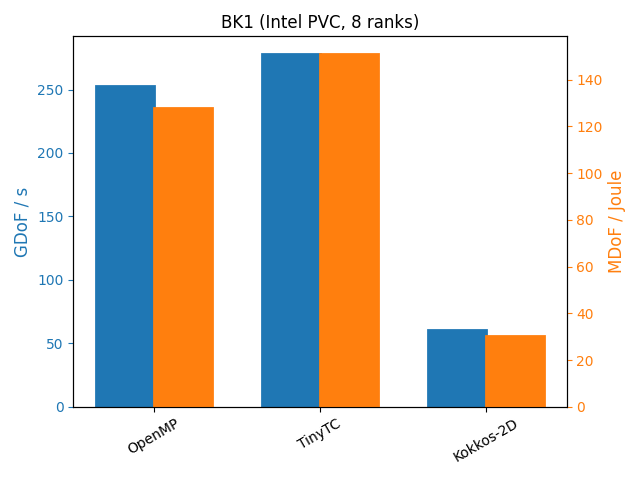
\includegraphics[width=0.5\textwidth]{figures/dealii_bk1.png}
    \caption{
            Performance (GDoF/s) and energy efficiency (DoF updates per Joule) of the OpenMP, Kokkos and TinyTC implementations of the BK1 mass operator, at the default operating point.
            % TODO: state device, polynomial degree, precision, problem size and driver/runtime versions.
    }
    \label{fig:intel_pvc_bk1_energy}
\end{figure}
